\chapter{Development}\label{ch:development}

\paragraph{Hardware testing} 

\section{Ultrasonic sensors} \label{us_test}

The first part of the hardware outline was testing of the ultrasonic sensors.
For each of the sensors a voltage divider was build as seen on figure /ref{voltage1}.

\begin{figure}[h]
\centering
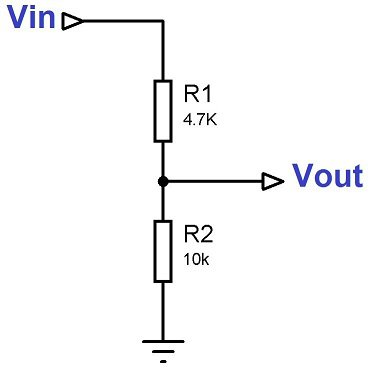
\includegraphics[width = 0.5\textwidth]{voltage1}
\caption{Voltage divider}
\label{fig::voltage1}
\end{figure}

The values of the resistors are calculated by the following equation:
\begin{equation} \label{voltagedivider} 
{V}_{out}={V}_{in}*{R}_{2}/({R}_{1}+{R}_{2})
\end{equation}

All sensors were tested out separately by connecting them individually to the Raspberry pi and running the test code below

\begin{lstlisting}
import RPi.GPIO as GPIO
import time
GPIO.setmode(GPIO.BCM)

TRIG = 23
ECHO = 24

print "Measuring distance"

GPIO.setup(TRIG, GPIO.OUT)
GPIO.setup(ECHO, GPIO.IN)

while True:
	GPIO.output(TRIG, False)
	print "Waiting for the sensor"
	time.sleep(2)

	GPIO.output(TRIG, True)
	time.sleep(0.00001)
	GPIO.output(TRIG, False)

	while GPIO.input(ECHO)==0:
		pulse_start = time.time()

	while GPIO.input(ECHO)==1:
		pulse_end= time.time()

	pulse_duration = pulse_end - pulse_start

	distance = pulse_duration * 17150
	distance = round(distance, 2)

	print "Distance:%d",distance

\end{lstlisting}

Each of the sensors worked as expected while connected separately, thus the logical progression was to test them out all at the same time.
While taking the readings, it was noticeable that some of the values where random or distorted due to noise and could not be used for accurate measurement. Therefore, some filtering had to be included in order to scale the values to an acceptable limit. A moving average filter was used for the previously mentioned task by taking three reading at a time and calculating the average of the values. 

\begin{lstlisting}
def readsensor(PIN):
	for x in range(0, 2):
		read_time_start1 = time.time()
		GPIO.output(TRIG, True)
		time.sleep(pulse)
		GPIO.output(TRIG, False)

		while GPIO.input(PIN)==0:
			pulse_start = time.time()

		while GPIO.input(PIN)==1:
			pulse_end= time.time()

		pulse_duration[x] = pulse_end - pulse_start
		time.sleep(0.05-(time.time()-read_time_start1))

	distance = sum(pulse_duration)/measurment_count* SPEED_OF_SOUND
	distance = round(distance, 2)
	print distance
while True:
	readsensor(ECHOF)
	readsensor(ECHOR)
	readsensor(ECHOL)
	
\end{lstlisting}

From the code above, the application of the moving average filter could be seen. Importantly there was a noticeable improvement of the readings, which became much more precise and consistent.
Furthermore, it can be seen that every reading takes less than 0.05 seconds. This is useful in making every cycle evenly long and predictable, when it comes to the total time that the program is required to run the full cycle. Therefore the time for the full sensor reading loop becomes $3\times0.05s=0,15s$.

\section{DC motors}
To make sure the purchased DC motors were operational an initial testing was performed by driving each of them in forward and in backward gear through the used driver. This can be seen in script below.

\begin{lstlisting}
GPIO.setmode(GPIO.BCM)
GPIO.setup(StepPinForward, GPIO.OUT)
GPIO.setup(StepPinBackward, GPIO.OUT)

def forward(x):
    GPIO.output(StepPinForward, GPIO.HIGH)
    print "forwarding running  motor "
    time.sleep(x)
    GPIO.output(StepPinForward, GPIO.LOW)

def reverse(x):
    GPIO.output(StepPinBackward, GPIO.HIGH)
    print "backward running motor"
    time.sleep(x)
    GPIO.output(StepPinBackward, GPIO.LOW)

print "forward motor "
forward(5)
print "reverse motor"
reverse(5)

print "Stopping motor"
GPIO.cleanup()

\end{lstlisting}

As it can be seen from the code, one of the motors was initially driven forward for 5 seconds and subsequently backwards for 5 seconds. To apply the test for the second motor simply the pin numbers(StepPinForward and StepPinBackward) were changed.

Furthermore, Pulse Width Modulation (PWM) was utilized in order to regulate the separate speeds of the motors, as it was an initial condition to implement cruise control.
in the final software what is ran on the device we have changed the forward() and reverse() so that we can change the speed of the motors at our desire.

\begin{lstlisting}
 def forward(forwardtime,SPEED):
	print "REVERSE"
	GPIO.output(StepPinBackward1, GPIO.HIGH)
	GPIO.output(StepPinBackward2, GPIO.HIGH)
	PWML.start(SPEED)
	PWMR.start(SPEED)
	time.sleep(forwardtime)
	GPIO.output(StepPinBackward1, GPIO.LOW)
	GPIO.output(StepPinBackward2, GPIO.LOW)
\end{lstlisting}

As you can see from the code above we use the drivers PWM input to change the speed of the vehicle.

\section{Raspberry Pi configuration and software}

In this section, a description of the steps taken to configure the Raspberry Pi, was made.

\subsection{Raspberry setup}

Initially, after obtaining the Raspberry Pi Zero, an installation of the Raspbian OS was performed.
Subsequently, all GPIO pins were enabled, followed by configuration of the Secure Shell (SSH) protocol in order to perform remote logins to the microcontroller. Furthermore, as mentioned in the Hardware chapter, due to it's size, the Raspberry Zero has only one USB port, resulting in a space limitation. Thus, the logical choice was to connect the Wi-Fi adapter to that USB port, and configure the microcontroller remotely, through the SSH. 
Additionally, extra tools such as Tmux Multitab and Nano Text Editor were used to clarify the programming sessions.

\subsection{Software}

The software constituting the robot's behaviour is self-made with the addition of several external libraries 

\begin{lstlisting}
import sys
import time
import RPi.GPIO as GPIO
\end{lstlisting}

To be precise, only three external libraries were used at the time of the development of this paper. Nevertheless, as the system is still in active development the list may expand after the submission of the documentation.

\begin{itemize}

\item \textbf{Sys module} \\ This module provides a number of functions and variables that can be used to manipulate different parts of the Python runtime environment. \cite{sys_module}

\item \textbf{Time module} \\ This module provides a number of functions to deal with dates and the time within a day. It is a thin layer on top of the C runtime library.
A given date and time can either be represented as a floating point value (the number of seconds since a reference date, usually January 1st, 1970), or as a time tuple. \cite{time_module}

\item \textbf{RPi.GPIO module} \\ This module is for functions that are connected to the GPIO pins.
\end{itemize}

The overall setup of the pins and the variables, with the different values used in the code, is present in the snippet below.

\begin{lstlisting}
#PIN numbers
LetfPWM=16
RightPWM=20
StepPinForward1=26
StepPinBackward1=19
StepPinForward2=13
StepPinBackward2=6
ECHOF=4
ECHOL=27
ECHOR=22
TRIG=17

#Values for reading the sesnsors
SPEED_OF_SOUND = 17150
measurment_count = 3
pulse = 0.00001	
pulse_duration = [0,0,0]
sensorF_data=0
sensorR_data=0
sensorL_data=0

#navigation variables
reversetime=0
turningtime = 1
MAXSPEED = 1
MEDSPEED = 0.6
MINSPEED = 0.1

#GPIO setup for each pin 
GPIO.setmode(GPIO.BCM)
GPIO.setup(StepPinForward1, GPIO.OUT)
GPIO.setup(StepPinBackward1, GPIO.OUT)
GPIO.setup(StepPinForward2, GPIO.OUT)
GPIO.setup(StepPinBackward2, GPIO.OUT)
GPIO.setup(ECHOF, GPIO.IN)
GPIO.setup(ECHOL, GPIO.IN)
GPIO.setup(ECHOR, GPIO.IN)
GPIO.setup(TRIG, GPIO.OUT)
GPIO.setup(LetfPWM, GPIO.OUT)
GPIO.setup(RightPWM, GPIO.OUT)

#PWM channels and frequency
PWML=GPIO.PWM(16, 0.5)
PWMR=GPIO.PWM(20, 0.5)
\end{lstlisting}

\subsection{Ultrasonic sensor reading}


As previously mentioned, the ultrasonic sensors are the proposed way of implementing collision detection. The desired function is for them to measure the distance from the robot to the closest present obstacle, and return the data for further usage in the code.
In subsection \ref{us_test}, it was mentioned of the potential problems with noise and the proposed filtering method, using the average of every three reading. 
Below is a section of the code, with the function for data acquisition after filtering the readings.

\begin{lstlisting}
 def readsensor(PIN):
	for x in range(0, 2):
		read_time_start1 = time.time()
		GPIO.output(TRIG, True)
		time.sleep(pulse)
		GPIO.output(TRIG, False)

		while GPIO.input(PIN)==0:
			pulse_start = time.time()

		while GPIO.input(PIN)==1:
			pulse_end= time.time()

		pulse_duration[x] = pulse_end - pulse_start
		time.sleep(0.05-(time.time()-read_time_start1))

	distance = sum(pulse_duration)/measurment_count* SPEED_OF_SOUND
	distance = round(distance, 2)
	print distance
	if PIN == ECHOF:
		sensorF_data=distance

	if PIN == ECHOR:
		sensorR_data=distance

	if PIN==ECHOL:
		sensorL_data=distance
\end{lstlisting}

The data reading is straightforward. The \textbf{TRIG} pin emits an ultrasonic impulse from a each of the sensors in addition to a digital timestamp that records the exact time of the event. When the impulse reaches back the sensor, a second timestamp is recorded. The logic behind it is that every loop should take equal amount of time for execution. 
The first timestamp in the beginning of the loop is initialized with \textbf{$read_time_start1 = time.time().$} and calculated afterwards in \textbf{$time.sleep(0.05-(time.time()-read_time_start1))$}. The expected cycle length is 0.05 second and is done to ensure that reading are acquired in the sensing range 0.02m to 4m.
The set time of 0.05 second is used, as it would give the range, limited by time.

\begin{equation}
330(m/s)*0.05s=16.5
\end{equation}

And since the impulse is going to the object in range and returning to the sensor, a division by 2 with give the max range for the time limitation 

\begin{equation}
16.5/2=8.25m
\end{equation}

The result is almost double the sensing range supported by the hardware. 

Furthermore, from the line: for x in range(0, 2): the reading of the sensor is done 3 times in a row, thus the implementation of the moving average filter.

The last lines of code ensure that when data reading is initiated, it would pass the value to only one of the readings, avoiding data collision.

\begin{lstlisting}
	if PIN == ECHOF:
		sensorF_data=distance

	if PIN == ECHOR:
		sensorR_data=distance

	if PIN==ECHOL:
		sensorL_data=distance

\end{lstlisting}

\subsection{Movements}

The expected movements of a differential drive robot was covered in section \ref{kin_analysis}. In this subsection, a description is conducted on the pre made functions governing the behaviour of the physical system. It is important to mention  
  
At the completion of this chapter, five different functions concerned with the movements, have been used.

The most basic function is the \textbf{stop()}, which as it's name suggests, halts the motion of the device

\begin{lstlisting}
def stop():
	GPIO.output(StepPinForward1, GPIO.LOW)
	GPIO.output(StepPinForward2, GPIO.LOW)
	GPIO.output(StepPinBackward1, GPIO.LOW)
	GPIO.output(StepPinBackward2, GPIO.LOW)
\end{lstlisting}

All the movement enabling pins will be set to low, which prompts the device to halt any ongoing movements. 

The second function is the forward motion.

\begin{lstlisting}
 def forward(SPEED):
	print "FORWARD"
	GPIO.output(StepPinForward1, GPIO.HIGH)
	GPIO.output(StepPinForward2, GPIO.HIGH)
	PWML.start(SPEED)
	PWMR.start(SPEED)
\end{lstlisting}

From the code snippet, it can be seen that when the forward function is executed, both of the motors start moving in the same direction and the speed is determined by the variable SPEED. It is important to mention that small fluctuations in the speed of each wheel will cause curved motion instead of the desired forward linear motion, as discussed in section \ref{kin_analysis}. Thus appropriate control needs to be applied in order to maintain equal speed in both wheels. 

How the speed is determined will be further discussed in subsection \ref{main_loop}: main loop.

The third function is the reverse, or what is essentially the same as the forward function only that the triggered pins are the backward ones. As in the forward movements, appropriate control is needed to maintain backward linear motion.

\begin{lstlisting}
 def reverse(SPEED):
	print "REVERSE"
	GPIO.output(StepPinBackward1, GPIO.HIGH)
	GPIO.output(StepPinBackward2, GPIO.HIGH)
	PWML.start(SPEED)
	PWMR.start(SPEED)
\end{lstlisting}

The two movements: forward and backward are the essential functions for the robot's linear motion.

Next we have the turning functions left() and right().
It was decided that the turning functions should be made that the vehicle takes the least amount of space to turn.
As it was explained in section \ref{kin_model},in a differential drive if the velocities of each wheel are the same but in a different direction, the robot will rotate around its middle point of the wheel axis, which essentially becomes the turning radius.

Below are the two functions needed for turning.

\begin{lstlisting}
 def right(turningtime,SPEED):
	print "RIGHT"
	GPIO.output(StepPinBackward1, GPIO.HIGH)
	GPIO.output(StepPinForward2, GPIO.HIGH)
	PWML.start(SPEED)
	PWMR.start(SPEED)
	sleep(turningtime)
	GPIO.output(StepPinBackward1, GPIO.LOW)
	GPIO.output(StepPinForward2, GPIO.LOW)

def left(turningtime,SPEED):
	print "LEFT"
	GPIO.output(StepPinForward1, GPIO.HIGH)
	GPIO.output(StepPinBackward2, GPIO.HIGH)
	PWML.start(SPEED)
	PWMR.start(SPEED)
	sleep(turningtime)
	GPIO.output(StepPinForward1, GPIO.LOW)
	GPIO.output(StepPinBackward2, GPIO.LOW)
\end{lstlisting}

As we can see both turns, right and left, are made with predetermined factor \textbf{turningtime}.
This will ensure that the vehicle will not over or under turn.
And since a decision was made to mount 3 ultrasonic sensors, the turning ratio on 90 degrees was found adequate.
Alteration of the turningtime will allow the device to turn to any desired amount of degrees, however a requirement of more than three ultrasonic sensors and specific positioning might be necessary.

\subsection{Main loop} \label{main_loop}

In this subsection the main loop, initiated when the device starts, is analysed.

\begin{lstlisting}
while True:
	readsensor(ECHOF)

	if sensorF_data>200:
		forward(MAXSPEED)
		
	if 200>sensorF_data>100:
		forward(MEDSPEED)

	if 100>sensorF_data>20:
		forward(MINSPEED)

	if 20>sensorF_data:
		stop()
		readsensor(ECHOR)
		readsensor(ECHOL)

		while sensorR_data<15 and sensorL_data<15:	
			reverse(MINSPEED)
			readsensor(ECHOR)
			readsensor(ECHOL)
			
		if sensorR_data>sensorL_data== True:
			right(1,MINSPEED)
			break
			
		if sensorL_data>sensorR_data==True:
			left(1,MINSPEED)
			break
\end{lstlisting}

The loop is initiated with reading of the front sensor \textbf{readsensor(ECHOF)}. Any further action is determined, based on the reading taken from it. If the distance to the closest object is over 2m the vehicle will start moving in a forward direction with full speed. When the distance drops down between 200 cm and 100 cm, the vehicle speed will be reduced to medium speed in order to prepare for a potential turning. Minimal speed is initiated when the distance from the front sensor drops down between 100cm and 20cm, allowing the robot to perform an instant stop. 
When the distance to the closet object falls under 20 cm,the vehicle will stop and will decide how to proceed based on 3 possible cases. The ultrasonic sensors on the left and right will estimate the distance to the closest object on both sides.

\begin{itemize}

\item Case 1 \\ If both sides fall under 15 cm of the closest object, the robot will perform reverse motion and constantly recheck if space becomes available on either side. Once that is true, the robot will perform appropriate turn. 
\item Case 2 \\ If one or both of the side sensors register distance to the closest object more than 15 cm, it will turn in the direction of the larger available space.
\item Case 3 \\ If the robot performs a turn with a minimal acceptable distance reading, it will re-evaluate the possible turning options.

\end{itemize}

After the turning phase the loop will go back to the beginning and start all over again.

The loop is made as simple as possible to avoid any complications while running the code.

\section{N.B.}

Unfortunately, due to shipping delays, the completion of this part was done without the acquisition of the optical encoders, necessary to implement the crucial wheel speed control. Obstacle avoidance was performed, relying on the similarity of the motors, and was sufficient to successfully test the above mentioned code. After the arrival of the encoders (which is after the completion of this paper),a thorough update would be performed on this chapter and presented in order at the examination date. 